
% This is misnamed filename. We wanted this to be the inrtoduction to
% the idea of adaptive runtime system

%\begin{frame}[fragile]
%\frametitle{An Empowered Runtime System}

%\begin{itemize}
%\item Think now, based on the model so far, what the runtime system
%  can do
%\item It is free to migrate chares across processors, as and when it pleases
%\item It is free to schedule the method invocations (including
%  constructors) that are waiting in the Queue on a processor in any
%  order it pelases
%\item Automatic Instrumentation
%\begin{itemize}
%\item It schedules invocations: so it knows how long they take
%\item It mediates communication: so it knows which chares talk to whom
%\end{itemize}
%
%\end{itemize}
%
%\end{frame}
%
%\begin{frame}[fragile]
%\frametitle{An Introspecitve and Adaptive Runtime System (CHANGE FIG)}
%\begin{itemize}
%\item Based on these capabilities, Charm++ runtime includes:
%\begin{itemize}
%\item Load balancing Schemes
%\item Fault Tolerance Schemes
%\item Communication optimizers
%\end{itemize}
%\end{itemize}
%
%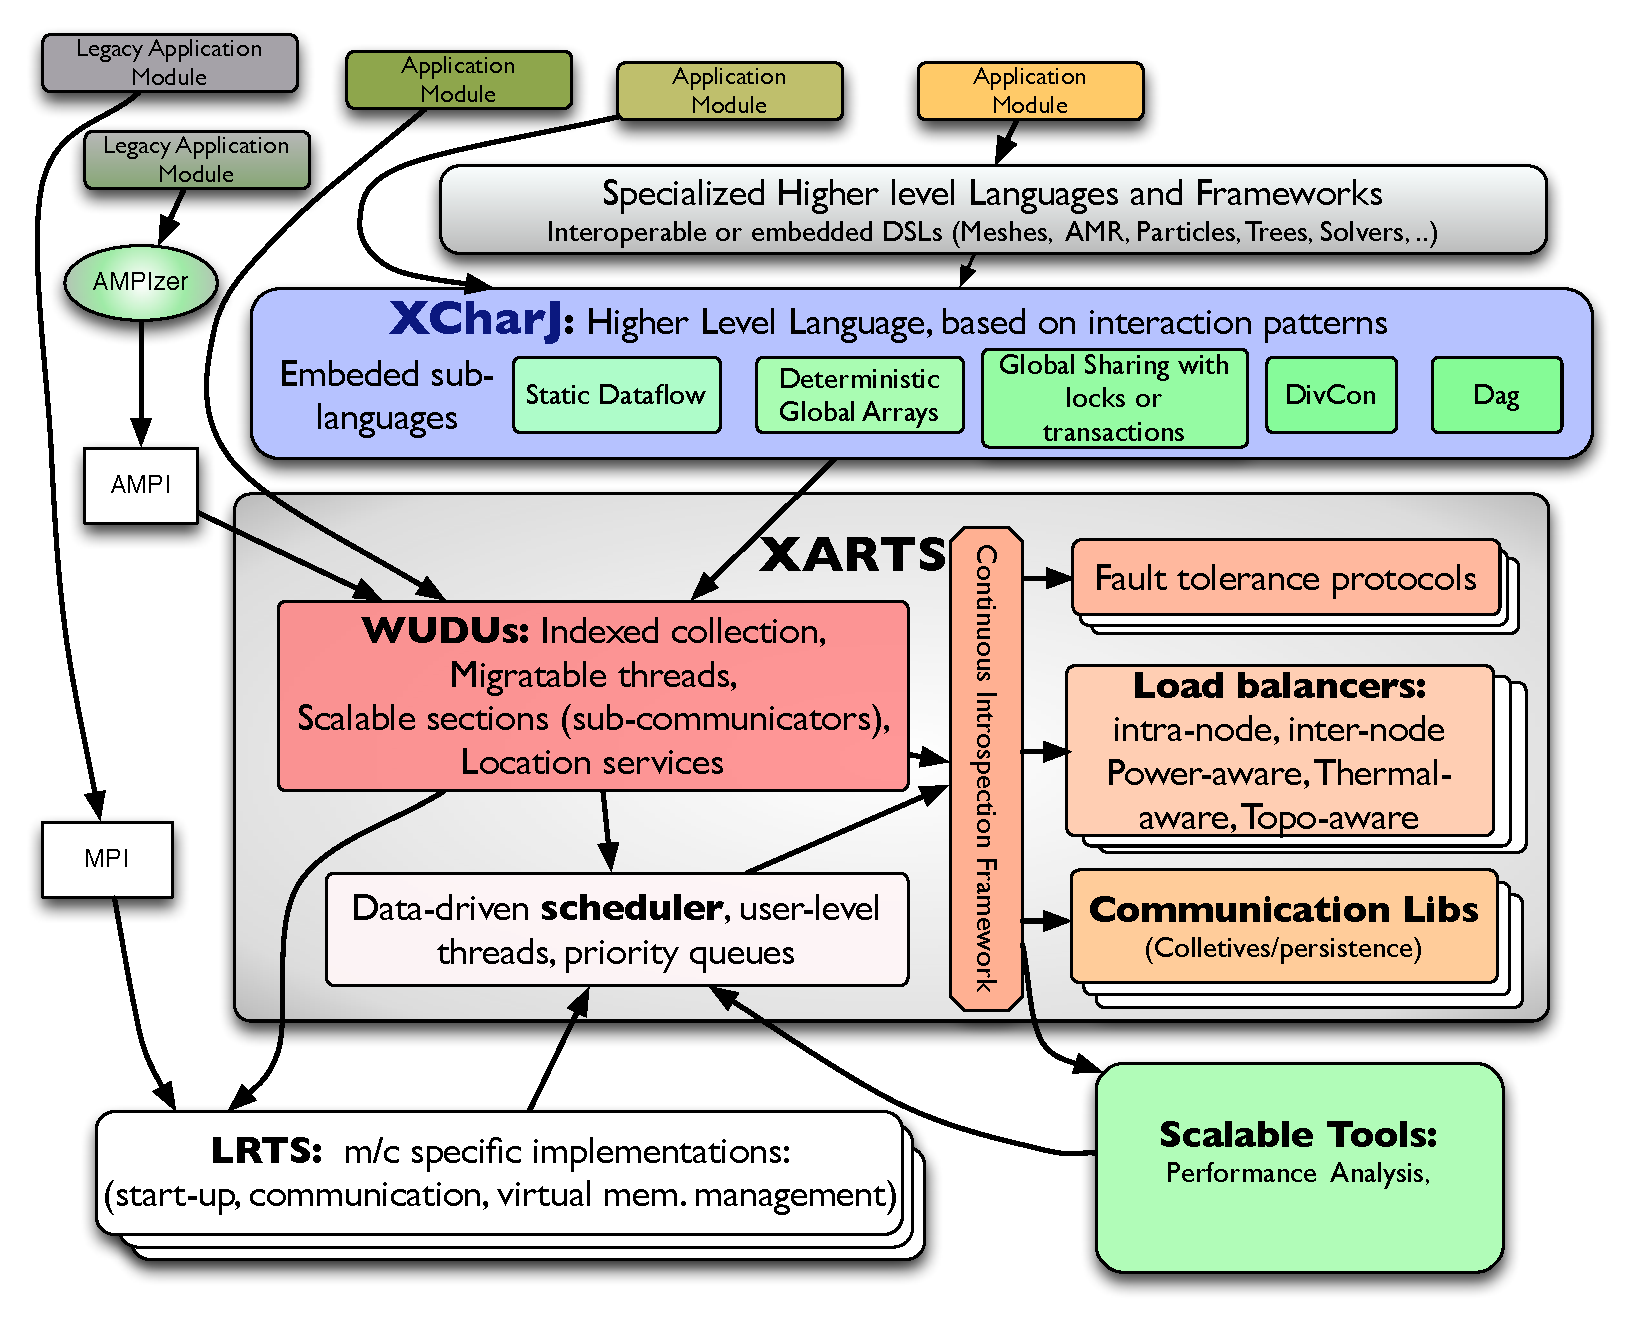
\includegraphics[width=0.8\textwidth]{figures/arts}
%
%\end{frame}

\begin{frame}[fragile]
\frametitle{Chare Migration: motivations}
\begin{itemize}
\item Chares are initially placed according to a placement map
\begin{itemize}
\item The user can specify this map
\end{itemize}
\item While running, some processors might be overloaded
\begin{itemize}
\item Need to rebalance the load
\end{itemize}
\item Automatic checkpoint
\begin{itemize}
\item Migration to disk
\end{itemize}
\item Chares are made serializable for transport using the Pack UnPack (PUP) framework
\end{itemize}
\end{frame}

\begin{frame}[fragile]
\frametitle{The PUP Process}
  \begin{center}
    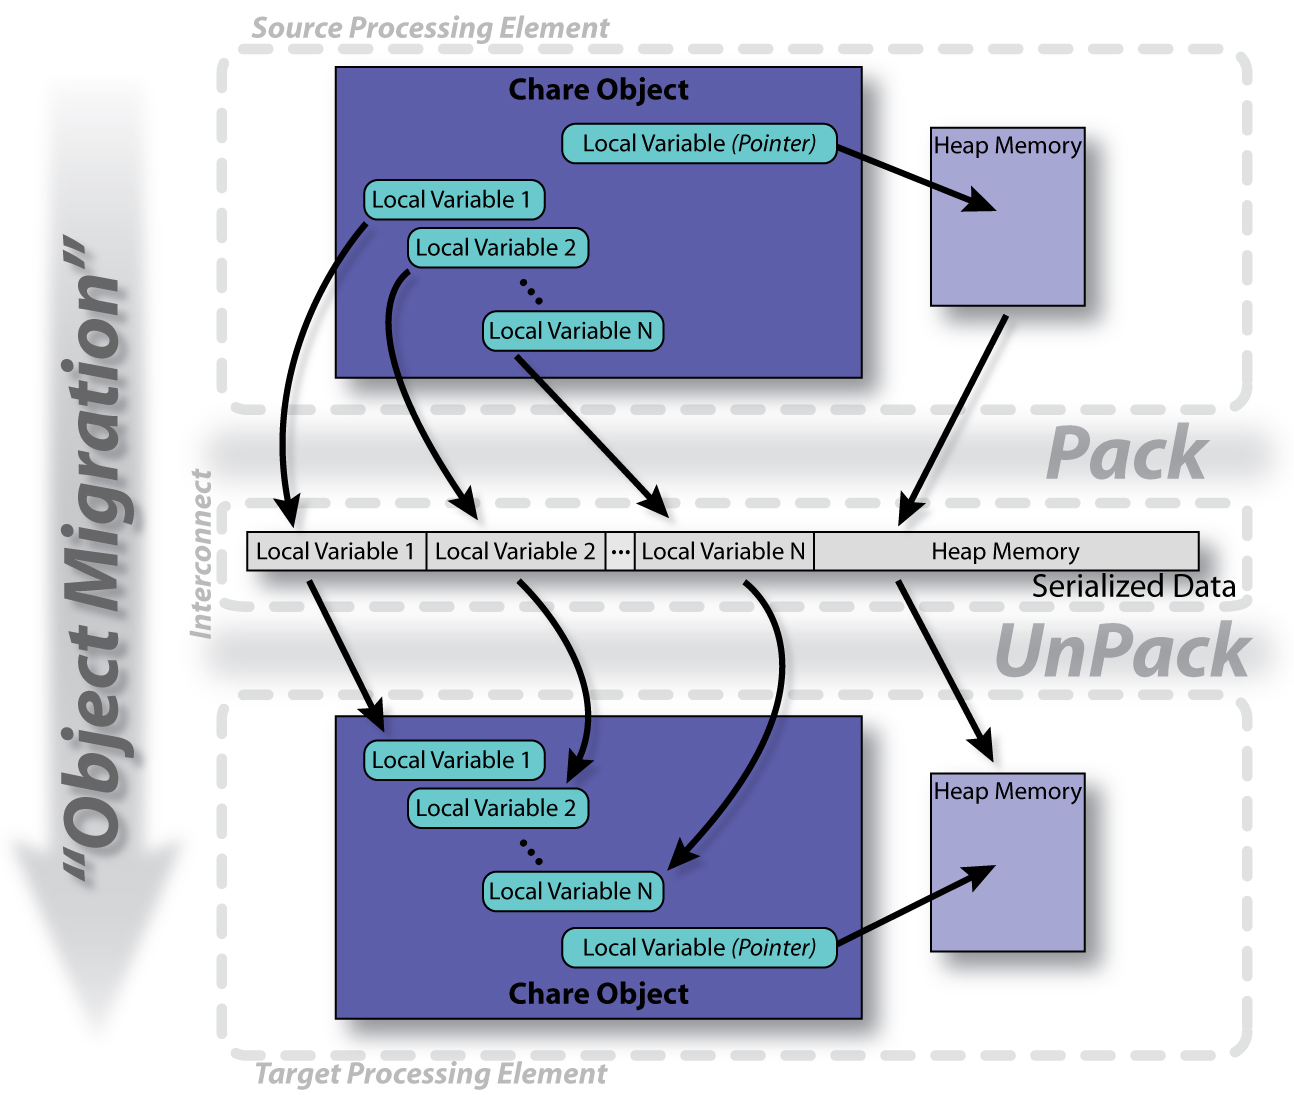
\includegraphics[width=0.8\textwidth]{figures/PUPProcess.png}
  \end{center}
\end{frame}


\begin{frame}[fragile]
\frametitle{PUP Usage Sequence}
  \begin{center}
    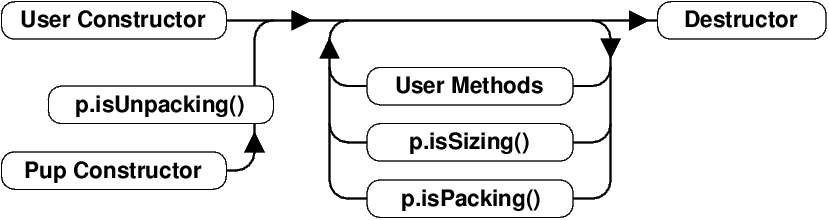
\includegraphics[width=0.8\textwidth]{figures/PUPUsage.png}
  \end{center}
\begin{columns}
 \begin{column}{0.5\textwidth}
 \begin{itemize}
 \item Migration out:
 \begin{itemize}
 \item ckAboutToMigrate
 \item Sizing
 \item Packing
 \item Destructor
 \end{itemize}
 \end{itemize}
 \end{column}
 \begin{column}{0.5\textwidth}
 \begin{itemize}
 \item Migration in:
 \begin{itemize}
 \item Migration constructor
 \item UnPacking
 \item ckJustMigrated
 \end{itemize}
 \end{itemize}
\end{column}
\end{columns}
\end{frame}

\begin{frame}[fragile]
\frametitle{Writing a PUP routine}
 \begin{columns}
 \begin{column}{0.5\textwidth}
   \begin{lstlisting}
class MyChare : public CBase_MyChare {
  int a;   float b;   char c;
  float localArray[LOCAL_SIZE];
  int heapArraySize;
  float* heapArray;
  MyClass *pointer;
 
  public:
   MyChare();
   MyChare(CkMigrateMessage *msg) {};
   ~MyChare() {
     if (heapArray != NULL) {
       delete [] heapArray;
       heapArray = NULL;
     }
};
 \end{lstlisting}
 \end{column}
 \begin{column}{0.5\textwidth}
  \begin{lstlisting}
void pup(PUP::er &p) {
   CBase_MyChare::pup(p);
   p | a;  p | b; p | c;
   p(localArray, LOCAL_SIZE);
   p | heapArraySize;
   if (p.isUnpacking()) {
     heapArray = new float[heapArraySize];
   }
   p(heapArray, heapArraySize);
   int isNull = (pointer==NULL) ? 1 : 0;
   p | isNull;
   if (!isNull) {
     if (p.isUnpacking()) pointer = new MyClass();
     p | *pointer;
   }
 }
}
  \end{lstlisting}
  \end{column}
  \end{columns}
\end{frame}

\begin{frame}[fragile]
\frametitle{PUP: Issues}
\begin{itemize}
\item If variables are added to an object, update the PUP routine
\item If the object allocates data on the heap, copy it recursively, not just the pointer
\item Remember to allocate memory while unpacking
\item Sizing, Packing, and Unpacking must scan the same variables in the same order
\item Test PUP routines with “+balancer RotateLB”
\end{itemize}
\end{frame}
